\documentclass[11pt, a4paper, twoside, openright]{book} %draft

\usepackage{graphicx,color}
\usepackage{amssymb, amsmath, array}



\begin{document}

% Example of title page for the projects carried out within the lasec 

% Simply include it in your mastex tex file: 
%        % Example of title page for the projects carried out within the lasec 

% Simply include it in your mastex tex file: 
%        % Example of title page for the projects carried out within the lasec 

% Simply include it in your mastex tex file: 
%        \input{cover}


% Updated March 2006 (SP)


\newcommand{\logoepfl}[0]{
  \begin{center}
    
\includegraphics[width=4cm]{logo_epfl_coul.eps}
  \end{center}
  \vspace{0.3cm}
  \hrule
}
\newcommand{\logolasec}[0]{
  \vspace{1cm}
  \hrule
  \begin{center}
    
\includegraphics[width=4.5cm]{logo_lasec_coul.eps}
  \end{center}
}
\newcommand{\project}[1]{
  \begin{center}
    \large{#1}
  \end{center}
  \vspace{1cm}
}
\newcommand{\department}[1]{
  \begin{center}
    \large{#1}
  \end{center}
}
\newcommand{\supervisor}[3]{
  \begin{center}
    \begin{normalsize}{
        \bf #1}\\#2\\#3
    \end{normalsize}
  \end{center}
}
\renewcommand{\author}[1]{
  \begin{center}
    \Large{#1}
  \end{center}
  \vspace{0.5cm}
}
\renewcommand{\title}[1]{
  \vspace{3cm}
  \begin{center}
    \huge{#1}
  \end{center}
  \vspace{1.7cm}
}
\renewcommand{\date}[2]{
  \begin{center}
    \normalsize{#1 #2}
  \end{center}
  \vspace{0.5cm}
}


\thispagestyle{empty}


% begin title page
  \logoepfl
  
  \title{Privacy Preserving Group Ranking}
  
  \author{Marc Ilunga Tshibumbu Mukendi}
  \department{School of Computer and Communication Sciences}
  \project{Semester Project}
  
  \date{June}{2016}

  \begin{center}
    \begin{tabular}{cc}
      \begin{tabular}{p{4.0cm}}
        \supervisor{Responsible}{Prof. Serge Vaudenay}{EPFL / LASEC}
      \end{tabular}&
      \begin{tabular}{p{4.0cm}}
        \supervisor{Supervisor}{Handan Kilinç}{EPFL / LASEC}
      \end{tabular}
    \end{tabular}
  \end{center}

\logolasec
% end title page




% Updated March 2006 (SP)


\newcommand{\logoepfl}[0]{
  \begin{center}
    
\includegraphics[width=4cm]{logo_epfl_coul.eps}
  \end{center}
  \vspace{0.3cm}
  \hrule
}
\newcommand{\logolasec}[0]{
  \vspace{1cm}
  \hrule
  \begin{center}
    
\includegraphics[width=4.5cm]{logo_lasec_coul.eps}
  \end{center}
}
\newcommand{\project}[1]{
  \begin{center}
    \large{#1}
  \end{center}
  \vspace{1cm}
}
\newcommand{\department}[1]{
  \begin{center}
    \large{#1}
  \end{center}
}
\newcommand{\supervisor}[3]{
  \begin{center}
    \begin{normalsize}{
        \bf #1}\\#2\\#3
    \end{normalsize}
  \end{center}
}
\renewcommand{\author}[1]{
  \begin{center}
    \Large{#1}
  \end{center}
  \vspace{0.5cm}
}
\renewcommand{\title}[1]{
  \vspace{3cm}
  \begin{center}
    \huge{#1}
  \end{center}
  \vspace{1.7cm}
}
\renewcommand{\date}[2]{
  \begin{center}
    \normalsize{#1 #2}
  \end{center}
  \vspace{0.5cm}
}


\thispagestyle{empty}


% begin title page
  \logoepfl
  
  \title{Privacy Preserving Group Ranking}
  
  \author{Marc Ilunga Tshibumbu Mukendi}
  \department{School of Computer and Communication Sciences}
  \project{Semester Project}
  
  \date{June}{2016}

  \begin{center}
    \begin{tabular}{cc}
      \begin{tabular}{p{4.0cm}}
        \supervisor{Responsible}{Prof. Serge Vaudenay}{EPFL / LASEC}
      \end{tabular}&
      \begin{tabular}{p{4.0cm}}
        \supervisor{Supervisor}{Handan Kilinç}{EPFL / LASEC}
      \end{tabular}
    \end{tabular}
  \end{center}

\logolasec
% end title page




% Updated March 2006 (SP)


\newcommand{\logoepfl}[0]{
  \begin{center}
    
\includegraphics[width=4cm]{logo_epfl_coul.eps}
  \end{center}
  \vspace{0.3cm}
  \hrule
}
\newcommand{\logolasec}[0]{
  \vspace{1cm}
  \hrule
  \begin{center}
    
\includegraphics[width=4.5cm]{logo_lasec_coul.eps}
  \end{center}
}
\newcommand{\project}[1]{
  \begin{center}
    \large{#1}
  \end{center}
  \vspace{1cm}
}
\newcommand{\department}[1]{
  \begin{center}
    \large{#1}
  \end{center}
}
\newcommand{\supervisor}[3]{
  \begin{center}
    \begin{normalsize}{
        \bf #1}\\#2\\#3
    \end{normalsize}
  \end{center}
}
\renewcommand{\author}[1]{
  \begin{center}
    \Large{#1}
  \end{center}
  \vspace{0.5cm}
}
\renewcommand{\title}[1]{
  \vspace{3cm}
  \begin{center}
    \huge{#1}
  \end{center}
  \vspace{1.7cm}
}
\renewcommand{\date}[2]{
  \begin{center}
    \normalsize{#1 #2}
  \end{center}
  \vspace{0.5cm}
}


\thispagestyle{empty}


% begin title page
  \logoepfl
  
  \title{Privacy Preserving Group Ranking}
  
  \author{Marc Ilunga Tshibumbu Mukendi}
  \department{School of Computer and Communication Sciences}
  \project{Semester Project}
  
  \date{June}{2016}

  \begin{center}
    \begin{tabular}{cc}
      \begin{tabular}{p{4.0cm}}
        \supervisor{Responsible}{Prof. Serge Vaudenay}{EPFL / LASEC}
      \end{tabular}&
      \begin{tabular}{p{4.0cm}}
        \supervisor{Supervisor}{Handan Kilinç}{EPFL / LASEC}
      \end{tabular}
    \end{tabular}
  \end{center}

\logolasec
% end title page



\newpage

\section{Motivation}

\paragraph{}
Group ranking is a process used to find a the best candidate from a group. The process involves a party called the \textbf{\textit{initiator}} 
and others parties called \textbf{\textit{participants}}. 
The initiator usually has a vector of preferences on some attributes and the participants have vectors of values, each corresponding to the attributes sought after by the initiator. At the end of the process, one or more candidates with attributes best matching the initiator preferences will be selected.
This has many applications such as online marketing,
personal interest matching, job recruitment  and selecting candidates for medical experiment.

\paragraph{}
However, this process is more and more used in virtual environment in today's society and as a consequence privacy concerns emerge. A trivial approach to Group ranking would leak private informations about all the candidates even if some of the will not be picked at the end of the process. As an example online forms are used to carry such ranking. A naive implementation of the ranking would require that the candidates provide private information(i.e by answering questions on the form). Since some group ranking imply ranking candidates on based on sensitive information, such implementation of group ranking poses a problem to privacy. 
\paragraph{}
Given the necessity of group ranking in a wide range of real world's application and the need to preserve candidates privacy, is there a way to perform group ranking while preserving privacy of all the parties? How do we prevent candidates to learn informations about other candidates? How do we prevent candidates to learn information about the initiator and thus cheating in the process? This is the subject of this paper.

In this report we present and explain a protocol
 %TODO : Put reference to paper here

that performs privacy preserving group ranking and we give a Java implementation of the protocol.

\newpage

\section{The protocol}

\paragraph{}
In this section we give a detailed explanation of the protocol. 

\subsection{Framework}
 The protocol is executed cooperatively by  \textit{n} + 1 parties. An initiator plus n Participant P0, P1... Pn. The protocol assumes that the participants are willing to accept the initiator invitation and to submit their private information if selected eventually.
The questionnaire given by the initiator is represented as a m-dimensional vector. The initiator holds a m-dimensional vector v0 indicating the preferred values of each of the question of the questionnaire, another m-dimensional vector represents the weight associated to each questions. Furthermore, the questionnaire comprises: "Equal" questions meaning that the initiator is looking for a specific attribute. "Greater than" question means that the initiator is looking for values exceeding some threshold. We assume without loss of generality that the first t questions are"greater than" questions. Finally the answer of each candidates is also represented by a m-dimensional Vector. A complete description of the protocol framework is given below:

\begin{figure}
	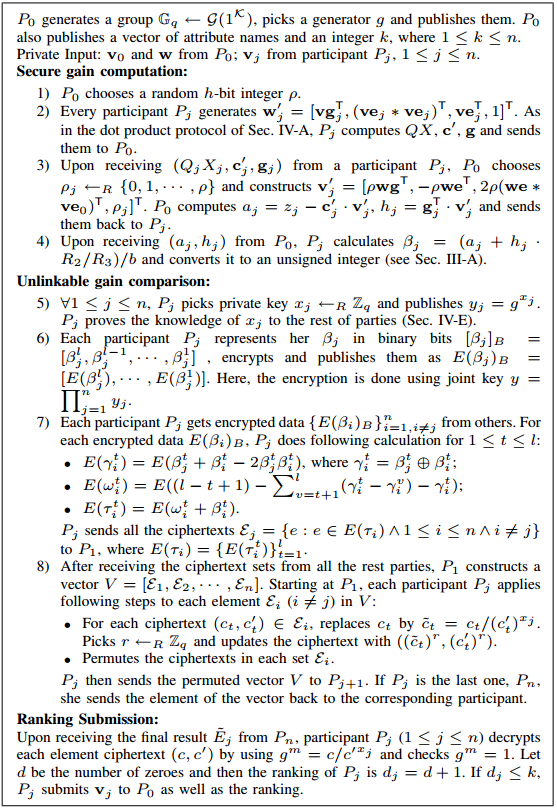
\includegraphics[width=\linewidth] {framework.png}
	\caption{Framework}

\end{figure}


\paragraph{Explanation of the protocol}
In our implementation, the same group will be used for every iteration of the protocol. The implementation uses a prime-order group of at least 1024 bits, thus the computation of discrete log is made difficult. 

\paragraph*{Secure gain computation}
First we define what is the gain in the context of this protocol.\\
%Make reference to paper
Given a criterion vector v0 = [v01, v02,..., v0m] and the weight vector w=[w1,w2,...,wm]. The partial gain value of Pj is \\
pj = $\sum_{k=t+1}^{m} wkv_{k}^{j}$ - $\sum_{k=1}^{t} (w_{k}(v_{k}^{j})^{2} - 2w_{k}v_{k}^{j}v_{k}^{0})$
In terms of dot products, the partial gain is given by $wg\cdot vg_{j} - we\cdot (ve_{j}*ve_{j})+2(we*ve_{0})\cdot ve_{j}$
\end{document}
